%%%%%%%%%%%%%%%%%%%%%%%%%%%%%%%%%%%%%%%%%%%%%%%%%%%%%%%%%%%%%%%%%%%%%
%%%
%%% Set these variables appropriately
%%%
\newcommand{\AUTHORS}{\normalsize{Harry Kalodner, Miles Carlsten, Paul Ellenbogen, Joseph Bonneau, Arvind Narayanan}\\
\normalsize{Princeton University}}
\newcommand{\TITLE}{An empirical study of Namecoin\\
and lessons for decentralized namespace design}
\newcommand{\KEYWORDS}{}
\newcommand{\CONFERENCE}{}
\newcommand{\PAGENUMBERS}{yes}       % "yes" or "no"
\newcommand{\TOAPPEAR}{no}
%%%
%%%
%%%%%%%%%%%%%%%%%%%%%%%%%%%%%%%%%%%%%%%%%%%%%%%%%%%%%%%%%%%%%%%%%%%%%

%%%% Setup the document/page
\documentclass[pdftex,twoside,twocolumn,12pt,letterpaper]{article}
\usepackage{ifthen}

\ifthenelse{\equal{\PAGENUMBERS}{yes}}{%
\usepackage[nohead,
            left=1in,right=1in,top=1in,
            footskip=0.5in,bottom=0.75in     % Room for page numbers
            ]{geometry}
}{%
\usepackage[noheadfoot,columnsep=0.2in,
            margin=1in,centering,truedimen]{geometry}
}

\usepackage[hyphens]{url}
\usepackage{fancyhdr}
\usepackage[numbers,sort]{natbib}
\usepackage{xspace}
\usepackage{booktabs}
\usepackage{tabularx}
\usepackage[table]{xcolor}
\usepackage{subfigure}
\usepackage[T1]{fontenc}
\usepackage{textcomp}
\usepackage{mathptmx}   % Times + Times-like math symbols
\usepackage{courier}
\usepackage[scaled=0.92]{helvet}

\usepackage{color}
\usepackage[pdftex]{graphicx}
\ifthenelse{\isundefined{\wantBW}}{%
  \usepackage[colorlinks]{hyperref}%        % for online version
}{%
  \usepackage[pdfborder={0 0 0}]{hyperref}% % for paper (B&W) version
}

\newcommand{\URL}[1]{\url{#1}}
\usepackage{doi}
%%%%% Setup for PDF
\hypersetup{%
pdfauthor = {\AUTHORS},
pdftitle = {\TITLE},
pdfsubject = {\CONFERENCE},
pdfkeywords = {\KEYWORDS},
bookmarksopen = {true}
}

%\setlength{\parindent}{0pt}
%\setlength{\parskip}{0pt}
\renewcommand{\headrulewidth}{0pt}
\newcommand{\Paragraph}[1]{\vspace{-2ex}\paragraph{#1.}}
\setlength{\topmargin}{-.15in}

\ifthenelse{\equal{\PAGENUMBERS}{yes}}{%
  \pagestyle{plain}
}{%
  \pagestyle{empty}
}

\makeatletter\long\def\@makecaption#1#2{
   \vskip 10pt
   \setbox\@tempboxa\hbox{\textsf{#1: #2}}
   \ifdim \wd\@tempboxa >\hsize % IF longer than one line:
       \textsf{#1: #2}\par      % THEN set as ordinary paragraph.
     \else                      % ELSE  center.
       \hbox to\hsize{\hfil\box\@tempboxa\hfil}
   \fi}
\makeatother

\clubpenalty=10000  % Don't allow orphans
\widowpenalty=10000 % Don't allow widows

\title{\textbf{\TITLE}}
\author{\AUTHORS}
\date{}

% Compact itemize and enumerate.  Note that they use the same counters and
% symbols as the usual itemize and enumerate environments.
\def\compactify{\itemsep=0pt \topsep=0pt \partopsep=0pt \parsep=0pt}
\let\latexusecounter=\usecounter
\newenvironment{CompactItemize}
  {\def\usecounter{\compactify\latexusecounter}
   \begin{itemize}}
  {\end{itemize}\let\usecounter=\latexusecounter}
\newenvironment{CompactEnumerate}
  {\def\usecounter{\compactify\latexusecounter}
   \begin{enumerate}}
  {\end{enumerate}\let\usecounter=\latexusecounter}

\newcommand{\comment}[1]{\textcolor{red}{#1}}
\newcommand{\ignore}[1]{}

\newcommand{\xc}[1]{\mbox{\textit{#1}}}
\newcommand{\la}{\leftarrow}
\newcommand{\ra}{\rightarrow}
\newcommand{\somespace}{\hspace{0.1cm}}

\def\discretionaryslash{\discretionary{/}{}{/}}
\def\discretionarydot{\discretionary{.}{}{.}}
\def\discretionarycolon{\discretionary{:}{}{:}}
{\catcode`\/\active
\catcode`\.\active
\catcode`\:\active
\gdef\URLprepare{\catcode`\/\active\let/\discretionaryslash
                 \catcode`\.\active\let.\discretionarydot
                 \catcode`\:\active\let:\discretionarycolon
        \def~{\char`\~}}}%
\def\URL{\bgroup\URLprepare\realURL}%
\def\realURL#1{\tt #1\egroup}%

\newcommand{\eg}{{\em e.g.}, }
\newcommand{\ie}{{\em i.e.}, }
\newcommand{\etal}{{\em et al.\ }}

\def\check{\stackrel{{\scriptscriptstyle ?}}{=}}

\begin{document}
\maketitle

% -*-LaTeX-*-
% $Id: abstract.tex 70 2007-01-30 21:59:16Z nicolosi $
\newcommand{\hi}[1]{\textcolor{red}{#1}}


\begin{abstract}
Secure decentralized namespaces have recently become possible due to cryptocurrency technology. They enable a censorship-resistant domain-name system outside the control of any single entity, among other applications. Namecoin, a fork of Bitcoin, is the most prominent example. 

We initiate the study of decentralized namespaces and the market for names in such systems. Our extensive empirical analysis of Namecoin reveals a system in disrepair. Indeed, our methodology for detecting ``squatted'' and otherwise inactive domains reveals find that among Namecoin's roughly 140,000 registered domain names, a mere 29 are actively used. Further, we develop techniques for detecting transfers of domains in the Namecoin block chain and provide evidence that the market for domains is thin-to-nonexistent.

We argue that the state of the art in mechanism design for decentralized namespace markets is lacking. We propose a model of utility of different names to different participants, and articulate desiderata of a decentralized namespace in terms of this utility function. We use this model to explore the design space of mechanisms and analyze the trade-offs.

\end{abstract}

   
\section{Introduction}
\label{sec:intro}

{\bf Decentralized namespaces.} We initiate the study of {\em decentralized namespaces} from an economic perspective. A namespace, as we define it, is an online system that maps names to values. The Domain Name System (DNS) is the most prominent example.  A web service such as Twitter that allows users to claim usernames and create profiles can be thought of as implementing a namespace. To be memorable by humans, namespaces must support arbitrary user-chosen strings as names. To be secure, namespaces must map each name to the same value for all users and adversaries shouldn't be able to convince a user that any other value is correct.

The problem of {\em decentralized} namespaces has long been recognized as an important one. The DNS is a critical yet centralized component of the Internet and those who control it can alter the web for all users. The controversies around the shutdowns of {\tt wikileaks.org} and the 2011 domain name seizures by the U.S. DoJ and DHS illustrate why many researchers and activists have sought decentralized alternatives \cite{wikileaks}.

The above three properties --- security, user-chosen names, and decentralization --- are known as {\em Zooko's triangle} \cite{zooko}. Until 2011, designing a system that exhibited all three was conjectured to be {\em impossible} \cite{square}. The rationale was that enforcing the uniqueness of name-value mappings and a consistent view of the directory for all participants would require a centralized server or a hierarchy.

{\bf Cryptocurrencies and Namecoin.} Cryptocurrency technology enables building a namespace with all three properties. Put simply, the block chain is a global, distributed data structure that can be repurposed as a directory. {\em Miners} execute a consensus protocol to establish the state of the system and are incentivized to do so by mining rewards they receive in exchange for their participation. As long as a majority of miners --- weighted by computing power --- follow the protocol, all users will see a consistent view of the directory when they query it. This in turn gives the system, and hence the underlying currency, economic value, making miners' actions profitable to them.

{\em Namecoin} is a cryptocurrency that realizes a decentralized namespace. It is the first altcoin from Bitcoin with its own block chain. It offers the same features as Bitcoin with the addition of a name/value store that can be used to hold arbitrary data (see Section \ref{sec:background}). The name/value store supports various applications; primarily, Namecoin has been used for domain-name resolution for the `.bit' alternative TLD, and by the online identity service, OneName, which utilizes the Namecoin block chain to record data about its members.

Namecoin offers a novel solution to the technical challenges of decentralized namespaces. However, there are also economic challenges. These arise from the fact that even though namespaces theoretically support an infinite number of names, the supply of names that are memorable and meaningful to humans is scarce. Allocating these names to users is therefore a mechanism-design challenge. {\em The central thesis of this work is that this mechanism design challenge is far harder than realized.} A system that gets it wrong may ``work" in a narrow technical sense, but may not be useful to real users.

Specifically, there are several crucial questions to consider: how do we model the economic behavior of the users of a namespace and what are the goals of mechanism design for namespaces? How well does Namecoin succeed at attaining these goals and what are its limitations? If Namecoin is not the ideal design, can we analyze the design space as a guide to the creators of future decentralized namespaces?

{\bf Our contributions.} Along the above lines, we make the following contributions. We begin by proposing a model of utility of different names to different participants and articulating desiderata of a decentralized namespace in terms of this utility function (Section \ref{sec:model}). We highlight the difficulty of mechanism design even in a toy model and explain the importance of making the model more realistic by incorporating extensions such as time-varying preferences.

The central contribution of this paper is a thorough empirical analysis of the Namecoin ecosystem. We develop a series of criteria based on the block chain, network behavior, as well as content to distinguish active websites from parked or squatted names (Section \ref{sec:domains}). This allows us to iteratively filter our dataset of around 120,000 registered names in Namecoin, leaving a mere 28 that  are not squatted, and have nontrivial content.

We then delve deeper into the economics of names. Namecoin has a built-in ability to transfer names, which is a secure way to trade them using the block chain. However, it is not obvious which transactions correspond to such sales, as opposed to regular name updates. We develop a novel analytic technique to distinguish the two types of transactions and find evidence for about 250 transactions in the entire history of Namecoin that may represent sales of names (Section \ref{sec:methods}). Of course, it is possible that more sales have occurred off the block chain, but there doesn't appear to be a widely known marketplace for Namecoin names.

%%\hi {Next, we develop a model for estimating the value of a name based on characteristics such as its length, the frequency of the name (treated as a word) on web pages, the Alexa rank of the corresponding .com, and several other factors (Section \ref{sec:}). In addition to the obvious goal of algorithmically pricing names, we seek to understand what makes a name valuable in the Namecoin community. Since there is almost no price data on sales of names, we instead use the observations we can make on the block chain about how names are treated by their owners. We posit that several characteristics such as a name being registered early in Namecoin's history and being re-registered quickly after expiry are indicative of more valuable names. We find that \hi{[enumerate characterstics]} are correlated with markers of high value. The high level of variation we find in the estimated value of different names further underscores the scarcity of names and the need for careful mechanism design.}

Based on all the empirical evidence we present, we are left to conclude that the Namecoin ecosystem is dysfunctional. The vast majority of registered names represent squatting and there is little evidence of a secondary market for names. While there could be many factors that explain the lack of adoption, there appears to be clear room for improvements in the design to minimize squatting and other problems. To this end, in Section \ref{sec:design}, we explore the design space of decentralized namespaces and make recommendations.

{\bf Why study namespaces?} Although we find that the Namecoin ecosystem is in disrepair, studying namespaces is important. While it's plausible there is no widespread dissatisfaction with today's DNS causing users to seek censorship-resistant alternatives, the existence of such alternatives provides a valuable hedge against a potentially abusive central authority. Besides, domain names are just one application of namespaces. Centralized directories for user public keys have fared much less well than DNS, and the service OneName, which we discuss in Section \ref{sec:conclusion}, is an interesting alternative. And of course, the problems posed by namespaces are intellectually interesting to study. 
We think decentralized namespaces have many important applications, but their promise hasn't been realized so far. Our work helps understand why this might be and lays the groundwork for a more rigorous approach to building such systems.

















\section{Background}
\label{sec:background}

In this section we cover the background of Namecoin. We begin by looking at the history of the cryptocurrency and then explain why a block chain can be used for our definition of a namespace. We then proceed to discuss the technical design of Namecoin and the mechanisms used in the design. We conclude this section with a discussion about the applications of Namecoin.

\subsection{History}

Namecoin is an alternative cryptocurrency modeled after Bitcoin\cite{nakamoto2008bitcoin}. Furthermore, it is the first altcoin in the sense that it was the first to create its own block chain, separate from Bitcoin's.  Namecoin shares many similarities with Bitcoin, including the same method for proof-of-work, the same coin cap, the same block creation time, and all of the same transaction operations (with a few additions). Namecoin was inspired after discussions about a BitDNS\cite{bitdns} protocol using a block chain to manage a domain name lookup service. The idea behind this was that a central authority managing domain names, such as ICANN, requires too much trust in a single entity. Having a decentralized name system described by BitDNS provides resistance against a single point of failure. The first Namecoin block was mined in April 2011, and as of the writing of this paper, over 215,000 total blocks have been mined in the Namecoin system. Because of its similarities with Bitcoin, Namecoin was able to be merge-mined and has been merge-mined with Bitcoin since October 8, 2011. 

\subsection{Description of the Block Chain}
\cite{bonneau2014decentralizing}
Namecoin is minted and maintained by a decentralized peer-to-peer network. Namecoin transactions require the digital signature of the account holder to prevent theft, and every transaction is published in an append-only hash chain, called the block chain. The block chain can be extended with new transactions by any participant, and such participants (informally known as miners) may obtain newly minted Namecoin currency (NMC) and/or tips from the transactions for performing this function. Extensions to the block chain require a proof-of-work that rate-limits the process (to approximately an extension every ten minutes) which enables a steady inflation rate, ample competition among participants to extend the block chain, and adequate time to obtain and verify the history of the block chain for new participants. Informally, the proof-of-work protocol in Namecoin is intended to maintain the following two essential properties about the block chain:

\begin{itemize}

  \item Every party eventually agrees on the order and correctness of transactions in the block chain.
  \item Any party can publish a transaction (for a fee), which will then be verified and, if valid, included in the block chain within a small bounded delay

\end{itemize}

A use case for a block chain is a tamper-evident log. That is, it can be used as a data structure that stores a bunch of data, and allows users to append data onto the end of the log. Each new block has a hash of the previous block, so if somebody alters data that is earlier in the log, it will be detected. If an adversary wants to tamper with data anywhere in this entire chain, in order to keep the story consistent, he's going to have to tamper with the hash pointers all the up to and including the current block. Thus it emerges, that by just remembering this single hash pointer of the head of the chain, users essentially remember a tamper-evident hash of the entire list, all the way back to the genesis block. Namecoin, and all block chain based cryptocurrencies, use this tamper-evident log in order to record all the transactions between individuals. 


{\bf Block chain security.}
The value and stability of a cryptocurency are directly related to the amount of proof-of-work involved in the calculations of the blocks because this work is what keeps the data distributed and secure in the tamper-evident block chain. For both Bitcoin and Namecoin, the proof-of-work is shown by calculating the hash of a new block and a random nonce over and over until the calculated hash has a certain number of leading zeros. The number of leading zeros required by the hash is referred to as the difficulty threshold. Namecoin enjoys a very high difficulty threshold for the proof-of-work because it is similar to Bitcoin and supports merge mining with Bitcoin. This allows miners who are mining Bitcoin to also mine Namecoin at the same time with no extra work for the miner. Essentially, this is because the miner is using their computational power to solve a cryptographic puzzle that satisfies the proof-of-work for both block chains at the same time. This is advantageous for the miners because they are rewarded with coins from both systems, and helps Namecoin because it gives the Namecoin network a vastly increased amount of hash power over what it would have if it did not support merged mining. The high hash power and difficulty of the cryptographic challenge on the Namecoin network increases the stability of the system, providing resilience to a 51\% attack and other threatening behaviors from malicious miners.

\subsection{Technical Details of Names}

In this section and the next, we make an effort to differentiate between the technical details of the Namecoin name/value implementation and the specific mechanism design choices in Namecoin. The feature that separates Namecoin from Bitcoin is that Namecoin is a namespace, and can be used to register name/value pairs that can be stored in the block chain and traded amongst individuals. This registration is done using the three script operations exclusive to Namecoin: {\tt NAME\_NEW}, {\tt NAME\_FIRSTUPDATE}, and {\tt NAME\_UPDATE}. In order to understand the registration process, we think it is helpful to walk through the registration process of {\tt name}, roughly following Figure \ref{fig:registration}. 

{\bf NAME\_NEW.}
To start, the user will need to select a coin to be crafted into a token (or special coin) that represents a name and whose value can be changed by whoever possess the token. The next step to register a name is to make a transaction that uses the {\tt NAME\_NEW} script operation in a transaction sending the token from one of their addresses to another. Using {\tt NAME\_NEW}, a user can indicate an interest in {\tt name} for a name/value pair by posting a hash commitment of the desired {\tt name} in the scriptPubKey of the transaction. The {\tt NAME\_NEW} operation acts as a signal in the block chain for name parsers to indicate that the next part of the scriptPubKey will be the hash commitment to a name. The protocol then places an {\tt OP\_2DROP} on the stack to remove all of the name information put on the stack with the {\tt NAME\_NEW} operation so that the rest of the locking portion of the scriptPubKey can function just as it does in Bitcoin. 

\begin{figure*}
  \centering
  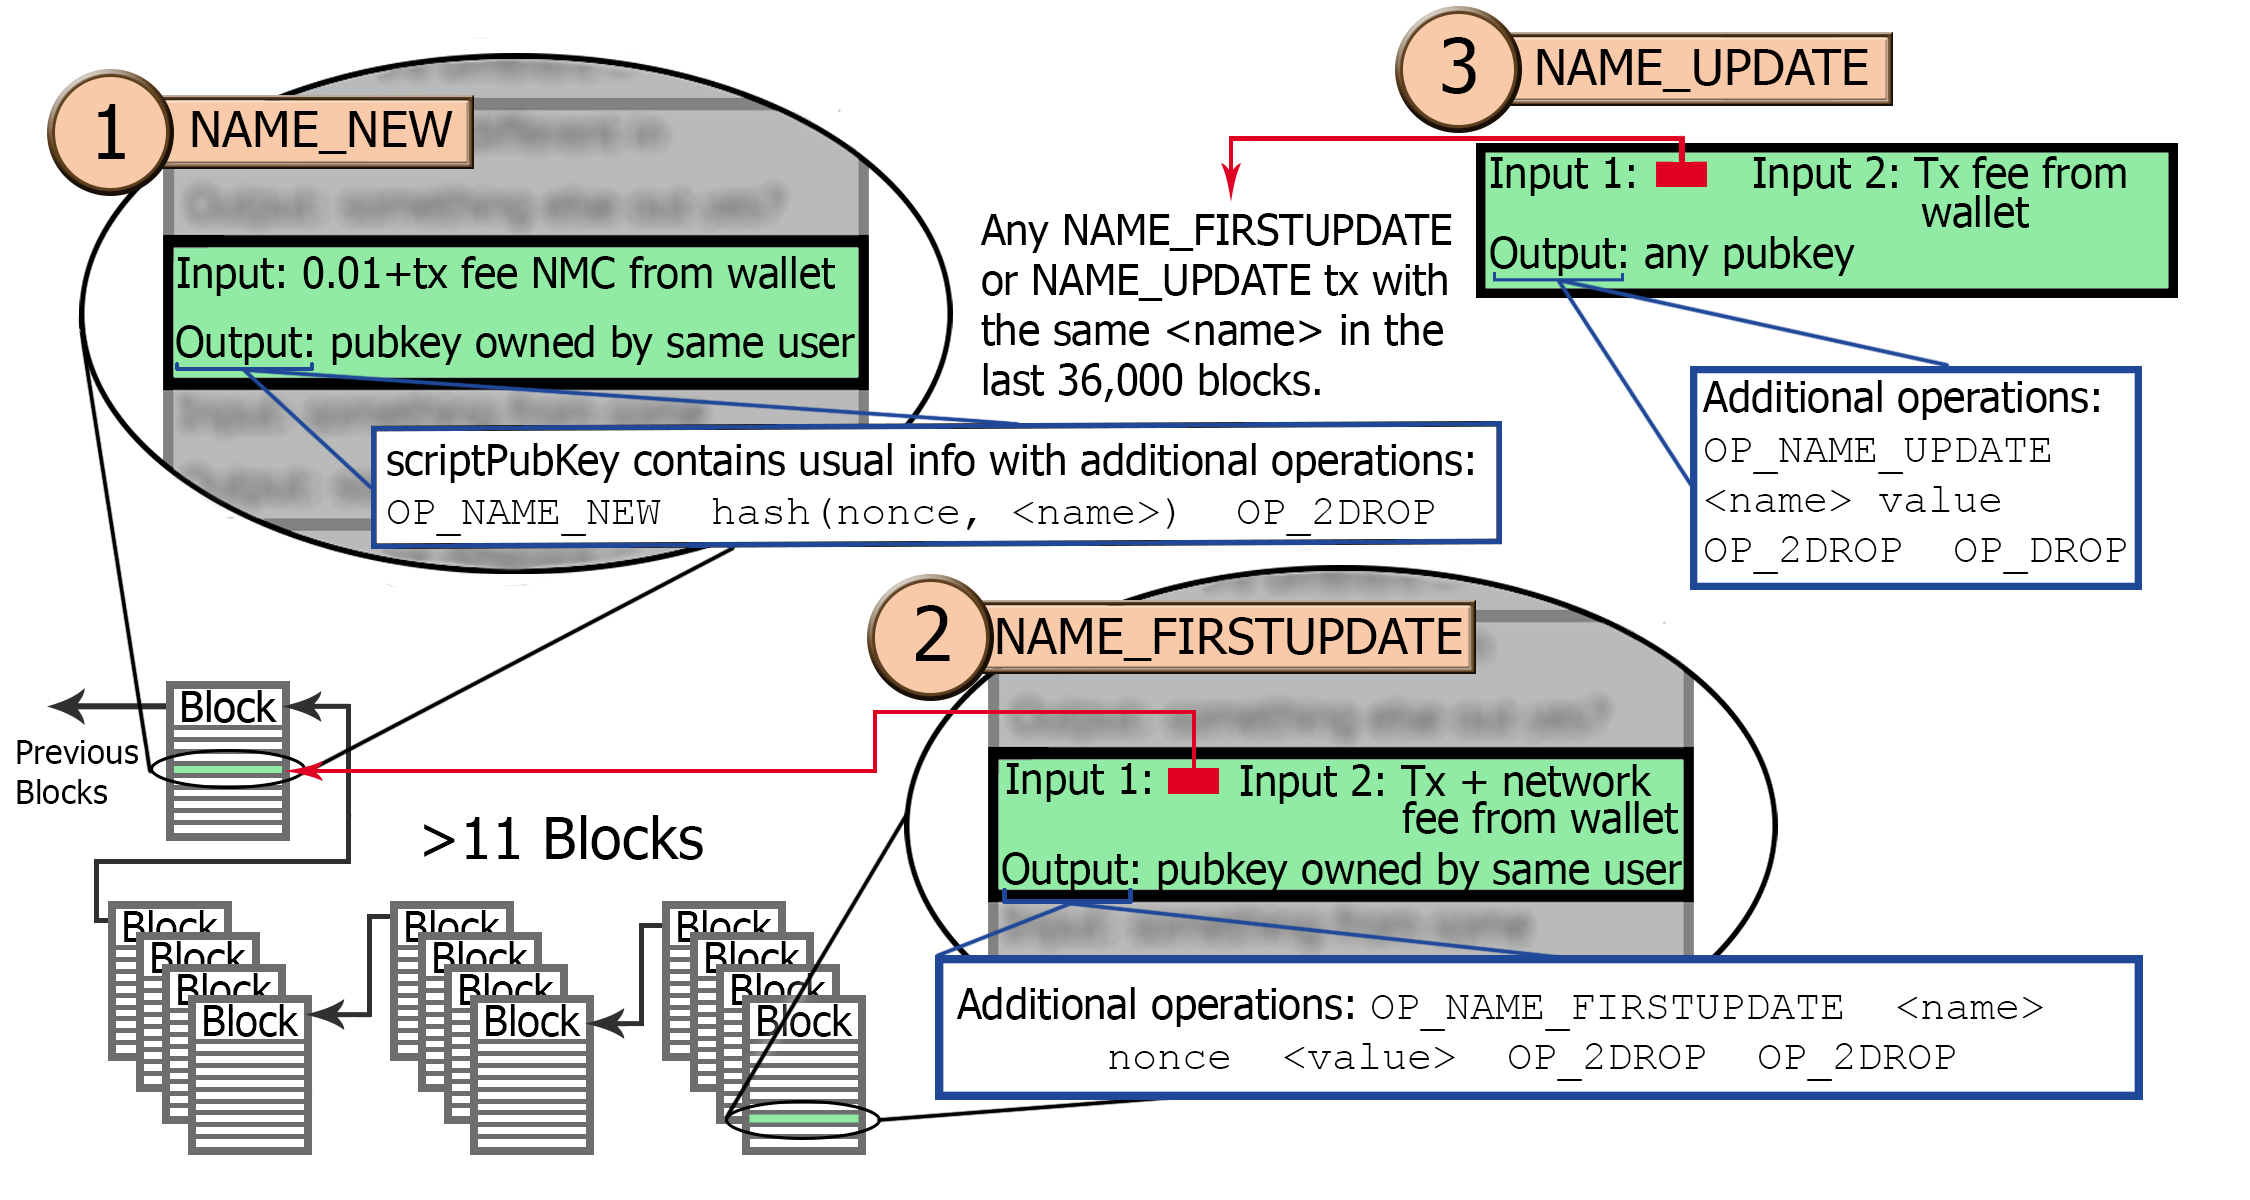
\includegraphics[width=0.95\textwidth]{figures/registration.png}
  \caption{Namecoin Name Registration Protocol}
  \label{fig:registration}
\end{figure*}

{\bf NAME\_FIRSTUPDATE.}
After doing this, and waiting for 12 or more blocks on top of the one containing the {\tt NAME\_NEW} transaction, the same user can use the output of the {\tt NAME\_NEW} transaction as the input for the {\tt NAME\_FIRSTUPDATE} transaction. Once completed, this will associate the chosen {\tt name} with {\tt value} selected by the user. Similar to {\tt NAME\_NEW}, {\tt NAME\_FIRSTUPDATE} allows data to be posted in the block chain as part of the scriptPubKey of a special transaction. 
To create a {\tt NAME\_NEW} transaction, a user will select, as input, the output of the {\tt NAME\_NEW transaction}. They will then use another address they control as the output for the transaction. The scriptPubKey of this transaction will contain a {\tt NAME\_FIRSTUPDATE}, the {\tt name} desired, the random nonce used in the {\tt NAME\_NEW} hash commitment, the first {\tt value} for the name to take and some {\tt OP\_DROP}s to clear these items from the stack so that they don't interfere with the rest of the locking script, which comes after these extra components. In order for this transaction to be valid, a miner will verify that the {\tt name} and the provided nonce do, in fact, hash to the commitment in the appropriate {\tt NAME\_NEW} transaction. The output of this transaction now contains the token representing the name/value pair for {\tt name} and {\tt value}, and whoever can unlock and spend the output can utilize the final new operation, {\tt NAME\_UPDATE}.

{\bf NAME\_UPDATE.}
The third and final new operation in Namecoin is the {\tt NAME\_UPDATE} operation. Again, this operation's arguments (the {\tt name} and {\tt newValue}) are stored in the scriptPubKey of a special transaction. This transaction must have as input a {\tt NAME\_FIRSTUPDATE} or {\tt NAME\_UPDATE} output with the same {\tt name}. This operation has three primary uses: updating, renewing and trading a name. If the user wants to change the {\tt value} associated with a given {\tt name}, they will update {\tt name} with this operation, providing a {\tt newValue}. If names can expire, as they do in Namecoin, then this operation can also be used to renew a name by providing a {\tt newValue} that is the same as the old {\tt value}. In either of these cases, the user will use an address they control as an output of the transaction. The final reason to make a {\tt NAME\_UPDATE} transaction is to trade the special coin to another user. In this case, the user will put, as an output, one of the other user's addresses instead of their own. Once the transaction resolves, the other user will have control over the special coin and can change the value to whatever they deem fit. Because the ownership of {\tt name} is associated with the ownership of the special coin, if the buyer is paying for the name with Namecoins, the exchange between the payment and the name can be atomic (meaning they happen in the same transaction and either are only valid if the other is as well). 

\subsection{Mechanism Design}

In this subsection we continue discussion about the details of Namecoin. As opposed to the last section, however, this section focuses on the specifics of the mechanism design in Namecoin. 

{\bf Fees.}
Namecoin has been implemented with various fees and protocols to incentivize the behaviours of the users. The special token used in the {\tt NAME\_NEW} transaction has a value of 0.01 NMC. This coin will be not be spendable like other Namecoins while it has a name attached to it, but if the name expires, then the coin will resume function as usual. For all of the transactions, {\tt NAME\_NEW}, {\tt NAME\_FIRSTUPDATE}, and {\tt NAME\_UPDATE}, the default behaviour is to have the user tip the miner. The current expected tip, which is programmed into the Namecoin client, is 0.005 NMC on each transaction. Historically, Namecoin also had a network fee attached to the {\tt NAME\_FIRSTUPDATE} transaction. The network fee is different from the transaction fee; the transaction fee is paid to the miners, whereas the network fee was destroyed (with an {\tt OP\_RETURN}) when a {\tt NAME\_FIRSTUPDATE} transaction was confirmed. The network fee varied over time-- it started at 50 NMC at the genesis block, but decreased by a factor of 2 every 8192 blocks (which is approximately 2 months). The purpose of the network fee was to have a large initial cost to claiming names to deter users from quickly claiming all the desirable names, but then decay off so that eventually the cost of registering a name becomes negligible. As of block 85585, the network fee became small enough that it rounds to 0 and is no longer added onto the transaction. The current implementation of Namecoin has no fees other than the transaction fees.

{\bf Expiration.}
Namecoin has an expiration time for names. Originally, the time period for a name to expire was 12,000 blocks, but by March 2012, the expiration period was increased to 36,000 blocks (which comes out to about 250 days). If a particular {\tt name} hasn't been mentioned in a {\tt NAME\_FIRSTUPDATE} or {\tt NAME\_UPDATE} in 36,000 blocks, the name becomes available again for any user to claim with {\tt NAME\_NEW} and {\tt NAME\_FIRSTUPDATE}. Similarly, a {\tt NAME\_UPDATE} must cite a {\tt NAME\_FIRSTUPDATE} or {\tt NAME\_UPDATE} that is less than 36,000 blocks old as input.

{\bf Changing the Protocol.}
Although it is difficult to change the protocol, it is not impossible and has already been done in Namecoin. Both the addition of merge mining with Bitcoin, and the increase in expiration length were not initially in the design of Namecoin. Both of these changes to the system required a hard fork in the block chain. In order to make these changes, the Namecoin community decided on arbitrary blocks at which point the new protocol would be enforced. For example, up to block 19,199 blocks that were merge mined with Bitcoin were not allowed into the Namceoin block chain, but starting on block 19,200 they were. 
 
\subsection{Applications}

There are many different subspaces in the Namecoin namespace, and the different subspaces have different applications. When claiming a name, a user prepends the name with a subspace ID and a slash. Namecoin was created to be very general so that it would be useful for any application that would benefit from an online name/value store. While {\tt d/} has the most registered names, there are many used subspaces in Namecoin.

{\bf .bit Domains.}
The vision for Namecoin was to use one of these subspaces for DNS lookup in the .bit TLD. Explicitly, Namecoin names associated with .bit domains are prepended with the subspace ID {\tt d/}. If a user wanted the domain awesome.bit, they would claim the name {\tt d/awesome}. The owner of awesome.bit would then set the value to their server address in a way that would be understood by .bit compliant DNS servers as described in the .bit specification\cite{bitdnsspec}.

Most major web servers, such as Apache, ngnix, and lighthttpd will accept connections through .bit domains with minor modifications to their per-site configuration files.

{\bf OneName.}

The name/value data store in Namecoin has applications beyond DNS. OneName is an online identity service that runs on top of Namecoin, making use of the data store. The idea behind OneName is that a user can have a name/value pair in the blockchain that associates said name with different online identities such as an email, GitHub, Twitter, and Bitcoin address. A OneName user can then confirm ownership of accounts on any of these services by referencing their OneName name through some messaging channel in each respective system. For example, if Alice wants to tie her twitter username to her OneName username, she must tweet the message ``Verifying that +Alice is my openname (my Bitcoin username). https://onename.com/Alice''. This is similar to the verification scheme Keybase uses. A OneName account also has an associated Bitcoin address so users can easily find an address to use to send Bitcoins to a particular individual, if they want.

In order to make a OneName identity, a user can visit OneName's website to create an account. A user makes an account by selecting a username and then optionally entering in their actual name, their account names, a short biography and picture, and a Bitcoin address. OneName takes the information given to it and automatically puts it into a name/value pair, with the name equal to the selected username, and the value containing all the other data. If the username is not already claimed by some user in the Namecoin subspace {\tt u/}, then OneName posts this pair into the blockchain. If it is already taken, the website will ask the new user to select a different username. If a user so desires, they can alternatively manually create a name transaction using the Namecoin client to create a name value pair with a name in the {\tt u/} subspace and a value formatted to match the OneName specifications. To incentivize using their website interface, OneName covers the Namecoin fees for their users. 





\section{Model}
\label{sec:model}

{\bf Names are scarce.} Many types of systems map keys or names to values. In his essay introducing his triangle, Zooko considers naming systems that include a system mapping PGP key fingerprints to keys. Fingerprints are hashes of keys. This would not qualify as a namespace by our definition because users cannot pick arbitrary names --- that would require finding the hash pre-image of an arbitrary name (fingerprint), a hard problem by the definition of a hash function. Zooko (and similar prior work) considers such systems to lack human memorability of names. We replace this criterion with that of user choice of names, which is roughly equivalent but easy to define rigorously. 

In a system that maps key fingerprints to keys, names are fungible and essentially infinite, and thus not scarce and have no market value. On the other hand, in any system that we call a namespace, scarcity is an almost inevitable consequence of free user choice. Even when names are scarce, the system architecture can make names more or less valuable. For example, usernames on Twitter are more valuable than on Facebook --- the username or handle is a relatively important way to find a user on Twitter, whereas on Facebook it is done more often by navigating the social graph.

The scarcity of names makes the design of namespaces challenging. But it also makes the problem particularly amenable to cryptocurrency-based solutions. Since names have market value, and participation in the primary market requires the associated cryptocurrency, the currency becomes valuable. This incentivizes miners, making the system secure.

{\bf The (non) role of trademarks.} Scarcity is also an issue in centralized namespaces, but it manifests in different ways. One key goal of most centralized systems is trademark protection. The trademark system can be seen as a legal solution to the problems of name scarcity and limits of human memorability in the real world, independent of any particular technological system. Most centralized systems support some form of arbitration or dispute resolution in which trademark plays a role.\footnote{For example see ICANN's Uniform Domain-Name Dispute-Resolution Policy \cite{}.} In a decentralized system, on the other hand, there is no easy way to enforce any rules that cannot be encoded algorithmically, and as yet there is no way to cryptographically assert that one is the owner of a trademark, and this may be impossible given the complexity and nuance of modern trademark law.

{\bf Primary and secondary markets.} We use the term primary market to mean the part of the market where new names are issued to users for the first time. By contrast, the secondary market deals with the sale of a name already in use. Perhaps the most technically straightforward way to implement the primary market is for names to be priced by the decentralized agent \hi{[elaborate]} encoded into the system, and for users to purchase names from this agent. The most straightforward implementation of a secondary market is to leave it entirely external to the system. This is the approach taken by Namecoin, but a variety of choices are possible. We elaborate in Section \ref{sec:design}.

{\bf Primary market pricing.} 

{\bf Squatting.} Even though names are scarce, it's not obvious what ``squatting'' means. After all, material goods are scarce, but we don't usually characterize car owners as squatting on them. The difference is that names have (vastly) different utility to different users. A squatted name is one that is owned by a user whose utility for that name is close to zero (or very small compared to the user who has the most utility for that name), purchased in hopes of selling to another user whose utility is higher.

Is squatting a problem for the system? This is a tricky question. If squatting exists merely because one side of the primary market is an algorithm and doesn't charge market price, then squatters could be seen as analogous to brokers or ticket scalpers. Such agents are sometimes considered to perform a useful market function \cite{}, or at least tolerated \cite{}, but not considered an existential threat to the functioning of the market.

On the other hand, squatters can be viewed as analogous to land speculators. This analogy is supported by the fact that names, like land but unlike tickets, are not fungible. The speculator may have zero utility for a name and makes no use of the name himself; he hopes that demand for a name will rise in the future, and may therefore not sell to a buyer who has a positive utility today. This could lead to a market failure in a few ways. The uncertainty around future demand means that some names may be squatted indefinitely, while legitimate users may end up with sub-optimal names. If most valuable names are locked up by squatters, it may prevent the growth of the sytem, in turn preventing the growth in market price for names that speculators are hoping for. Land speculation has also been criticized as contributing to a market failure \cite{archer73}. 


In this view, squatting may exist and may be problematic even if the primary market is able to discover the market price. But if the primary market is algorithmic, it only exacerbates the squatting problem.


{\bf Complexity of the utility function.} 
Our argument above is essentially that utility functions are time-varying. This is particularly relevant to cryptocurrency-based namespaces, since they need to ``bootstrap,'' \hi{[explain]} and many users may have a zero or negligible utility for all names until they decide to participate in the namespace at all.

Another aspect of complexity of the utility function is diminishing marginal utility. A user named John Smith may want either the name \textsf{JohnSmith} or \textsf{john-smith} but not necessarily both. Time-variation and diminishing marginal utility make the mechanism design problem very tricky.

Suppose, to the contrary, that utility functions are time invariant, and utility functions of a user for different names are independent. Then we may state the goal of the system as ownership of each domain by the user with the maximum utility (or willingness to pay) for that domain, as long as that value is above some threshold. We can easily realize this by making the primary market a second-price auction with a reserve price. No secondary market would be necessary.

Of course, this is oversimplified. Let's add diminishing marginal utility to this model. Suppose there are 10 John Smiths in the world and 10 variations of the name \textsf{JohnSmith}. A 10x10 matrix describes the utility of each user for each name. Further, none of these users has any utility for more than one name. Now we can state a welfare-maximization goal of finding the assignment of names to users that maximizes the sum of each user's utility for his assigned name, which translates to a maximum weighted graph matching problem. Or we could be happy with a Pareto-efficient assignment; since this is one-sided market (names aren't agents), this is the house allocation problem \cite{matching-markets-theory-practice}. This shows that even in a highly simplified setting with a finite number of names and the same number of users, the mechanism design question is very tricky.

When we add time-varying preferences to the model, it is unclear if we can even formally state a goal for the system. The harder we make it for a user to hold on to a purchased name, the easier it becomes for an adversary to ``seize'' a name (see below).

At any rate, the fact that preferences are time varying appears to be part of the reason that names in Namecoin expire and must be renewed; in effect, they are leased rather than purchased outright.

{\bf Seizures.} The Namecoin community considers it a major goal to prevent ``seizures'' of domain names by adversaries \cite{}. To prevent seizures, then, it must be easy to hold on to a name after buying it. This is in tension with preventing speculation, which works by buying a name and holding on to it despite other people wanting it.

The reason it is even technically possible to prevent such censorship in the face of a well-funded adversary is that the adversary can't possibly pre-emptively buy up all the names that the victim might use. For example, Wikileaks might find any name with the string ``wikileaks" in it to be acceptable, even if not ideal, for their purposes. In other words the victim's utility function has a large support; the adversary's utility for a name is {\em contingent on} the victim owning that name.


%It turns out that the utility of an adversary for a name can be predicated on the ownership of that name by a particular user. For example, a government may want wikileaks.bit to shut it down if Wikileaks owns it and is operating it, but otherwise may have a much smaller utility for that domain. (After all, the government couldn’t hope to pre-emptively buy up all the names that Wikileaks might use.) To prevent seizures, then, it must be easy to hold on to a name after buying it. This is in tension with preventing speculation, which works by buying a name and holding on to it despite other people wanting it.






\section{Domain Analysis}

\subsection{DNS Records}

In order to support DNS lookups, Namecoin provides a specification that allows for the support of most DNS record types. A name's configuration is stored in a JSON dictionary object which is placed in a name's value. Domain's can be configured in a number of different ways. The main methods are directly setting one of more IP (or IPv6) addresses or setting one or more secondary name-servers which hold information about a domain. Additionally records can link a name to a number of hidden services like .onion\cite{onion} and .i2p\cite{i2p}.

Namecoin supports a number of different name resolution methods. Different methods have different properties and thus it is interesting to inspect how people are setting up their domains. The vast majority of people are pointing their domains directly to an address. This includes people using IP, IPv6, and Tor. This is by far the most secure method since the IP address is protected directly with blockchain security. A user can simply look up a name in the blockchain and immediately be linked to a server. However, this security comes at the cost of flexibility since the server is directly encoded in the blockchain. and can not be changed without an update.

\begin{figure}
  \centering
  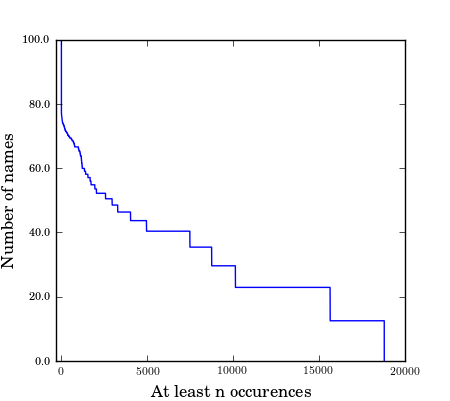
\includegraphics[width=0.9\columnwidth]{figures/squatters2}
  \caption{Namecoin Name Registration Protocol}
  \label{fig:registration}
\end{figure}


\begin{table}[t]
\begin{tabular}{ll}
Type of Resolution & Count \\ \hline
Nameserver URL     & 3359  \\
Nameserver IP      & 175   \\
Single IP          & 6304  \\
Multiple IP        & 3     \\
Single IPv6        & 3     \\
Multiple IPv6      & 1     \\
Tor                & 12    \\
Alias              & 27    \\
Only Subdomains    & 135   \\ \hline
Total              & 10019
\end{tabular}
\end{table}


%insecure delegation like DNSSEC
% cite DNS lookup attack
The much more flexible configuration, used by a large number of people as well, is nameserver delegation. Rather than directly listing an IP address in the blockchain, one or more nameservers are listed. This way a name owner can update it's IP address without modifying the blockchain. However this is insecure delegation since Namecoin can not enforce that the server provide everyone with the same content. Additionally if a nameserver is listed with a hostname rather than and IP address, a standard DNS lookup must occur. This lookup is very susceptible to attack and thus not a strong security option. However many more people are using nameserver URLs rather than IPs.

\subsection{Empirical Study}
\label{domainbreakdown}

\begin{table}[t]
\begin{tabular}{ll}
Active d/ Names     & 141422  \\
JSON Dictionary      & 48894   \\
Valid DNS          & 10118  \\
Curlable        & 5374     \\
Not Squatter        & 745     \\
Without Duplicates      & 455     \\
Without Errors              & 278    \\
With Content              & 223    \\
Without ICANN hostname   & 29   \\
\end{tabular}
\end{table}

In order to produce an accurate understanding of the current landscape of Namecoin domain names, we explore the status of the d namespace. Our goal is to measure content reachable through .bit domain names. The d/ namespace contains 141422 active names. We explore the content that these names hold.

We want to analyze web content being served by .bit domains, but trying to contact every single one of the 141422 active names would be a difficult and time consuming task. In order to cull this large number we look at the subset of names that have a chance of resolving. Simply limiting our search to only include names with values that are JSON dictionaries limits us to 48894 names.

To further reduce the number of domains we must query, we filtered these entries to include only those that have DNS information that could allow resolution of the domain. The Namecoin DNS Specification lists a number of fields which can be used to link a name with an IP address. We only queried names which included at least one of these fields. Additionally servers were removed if they pointed to a local or loopback IP address. After this we were left with 10118 domains.

We attempted to download the http front page of each of these 10118 names. 4645 of these domains were unreachable or didn't serve web content leaving us with only 5374 domains which present any response.

At this point we moved to looking at the content of server responses. Immediately noticeable was the fact that 4629 of these names pointed came from 3 different squatters. These domains held nothing of value and caused massive inflation in our reachable domain count.

Without the squatters, we had 745 viable domains. However many of these pages included identical content which does not add value to the system after removed 290 of such duplicates we had 455 domains left.

At this point we started inspecting the actual content of the webpages. A large number of them were either error responses from the server or default pages from various servers. Neither of these types of pages are usable content. Removing the 177 of these left us with 278 domains.

Out of the remaining sites, many had very small amounts of content consisting of only a few words on a blank page like, "Welcome to mysite.bit." These pages, though valid uses of Namecoin, do not provide any utility to a visitor. Thus we decided to look at only pages consisting of 14 or more words and images which brought us down to 223 pages.

These 223 pages make up the only websites reachable through .bit domain names which have real content on them at the time of this analysis. This represents the value of .bit domains to people who can visit them today. We are further interested in the subset of these pages which don't come from a server that is accessible through a standard ICANN TLD as well.  83 of the pages directly redirect the user to a standard domain and 111 were manually identified as pointing to the same site as a standard domain.

We finished our analysis with 29 pages remaining. These pages represent the .bit unique content available.

\subsection{Detecting Squatters}

Names are owned by individual addresses rather than by identities and it is common practice to keep each purchased name under a different address. Thus it is difficult to assess how many names a single person owns. However many squatters are easily identified through the values they set on names they own. Since there is no built-in mechanism for the marketing and sale of names built into Namecoin, squatters use the values of names they own to display contact information. This information generally comes in the form of either contact information stored directly in the value of a name, or contact information stored on the IP address to which the name resolves.

This behavior provides us with an easy facility to track the presence of squatters since a squatter's contact information is generally constant among all the names he owns. Thus evaluating the frequency of values on the blockchain at any given time, we can measure the rate of squatters compared to regular users.

There is no clear method for deciding exactly of often a value has to occur in order to assume a squatter has been detected. However even the coarsest grained approach displays the massive amount of squatting on the blockchain. Simply observing the 196023 currently active names, reveals that there are only 34361 unique values.

\subsection{Categorizing Squatter Name Decisions}

As we have seen, many individual squatters buy up very large numbers of domains. We now explore what sort of categories these names fall into and through this try to interpret the decisions these squatters have made. Surprisingly squatters do no follow many obvious strategies of name selection.

STUB
\section{Secondary market analysis}
\label{sec:methods}
Next, we seek to understand and quantify how names move between users. Our basic scenario is that Alice owns the name `d/example' and Bob would like to purchase it from her. We explore various ways this sale can occur and how these sales can be detected.

\subsection{Detecting atomic transfers}

\begin{figure*}
  \centering
  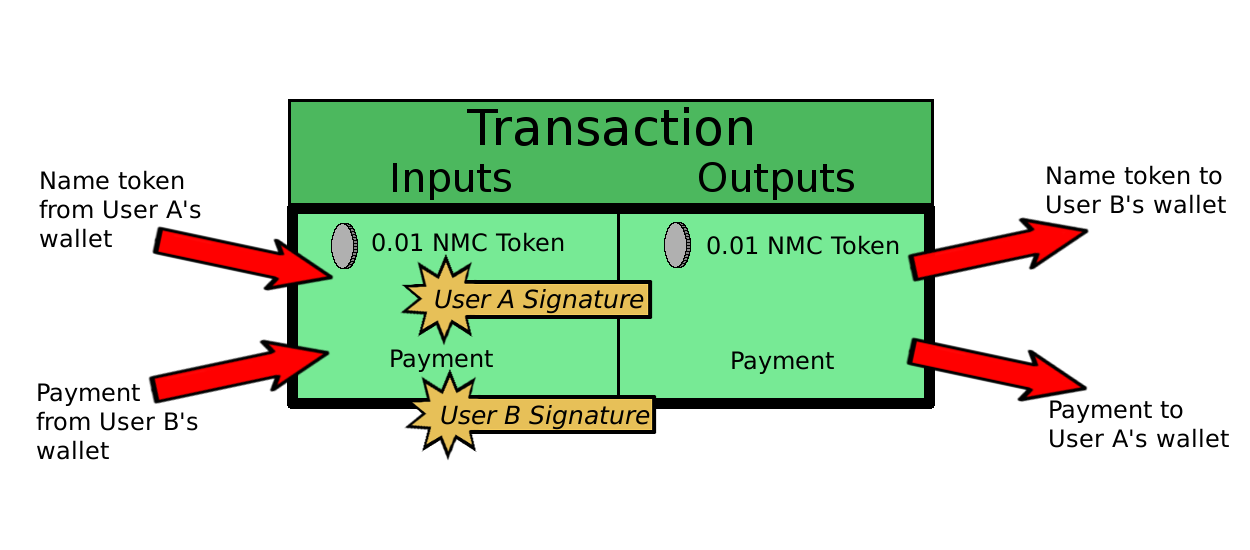
\includegraphics[width=0.9\textwidth]{figures/atomicTX}
  \caption{Anatomy of an atomic name transfer. Both the name and the payment are included in the same transaction, so one cannot fail to transfer to the other party without the other failing to transfer.}
  \label{fig:atomic}
\end{figure*}

The safest way to buy and sell Namecoin names is through the use of atomic transactions. This is an important technique in cryptocurrencies whereby two parties can exchange digital assets (such as a name in exchange for currency) without a trusted intermediary without either worrying that the other will abscond after receiving her half of the bargain. We show how these transactions work in Figure \ref{fig:atomic}. In an atomic transaction, Alice and Bob make their exchange in a single transaction. In the simplest form of atomic name transfer, Bob creates a transaction which transfers his payment to Alice and transfers `d/example' to him. He then sends this transaction to Alice, the owner of the name, who verifies it, signs, and broadcasts the transaction to the block chain. Both Alice and Bob's signatures are locked to the inputs and outputs of the transaction so neither input can be spent individually without the full transaction. This transaction provides cryptographic security to both Alice and Bob since either both the name and coins will be exchanged or nothing will. Although there is nothing inherently different looking about this transaction on the block chain, there are a few possible techniques to detect them by implementation quirks.

The Namecoin client is a fairly underdeveloped piece of software and thus there is no built-in method of performing atomic transactions. In order to accomplish this task, the Namecoin RPC client must be used from the command line. In order to simplify this task, a Namecoin developer created ANTPY \cite{antpy}, a piece of software to automate the creation of atomic transactions. This software has the quirk that the buyer's payment goes to the address that the seller held the name in. To find these transactions we queried the block chain for transactions with a {\tt NAME\_FIRSTUPDATE} or {\tt NAME\_UPDATE} input from the same address as a non name output. We then further reduced this set by eliminating transactions where the name stayed at the same address.

We searched throughout the history of the Namecoin block chain for transactions fitting this specification. Our query returned 13 transactions which we believe represent all transactions built by the ANTPY script. However this by no means represents all sales on the block chain. We next attempt to discover atomic transactions in a different way.

A implementation-agnostic method for detecting atomic name transfers is to find transactions that clearly use change addresses. This occurs when there are two non-name outputs in a transaction that has a name input. In this case the buyer did not want to pay all of his input to the seller and thus kept some for himself. This leaves the transaction with 3 outputs. Under normal circumstances, {\tt NAME\_UPDATE} transactions will only have two outputs, a name output and a change address. Thus every transaction with three outputs is very likely an atomic name transfer.

In the history of the Namecoin block chain, we found 6 transactions fitting this form. However 5 of the 6 were also detected by the previous (ANTPY) criterion.

The 14 atomic transactions which we detected are a lower bound for the number of name transfers. We are unable to query for all atomic transactions since if the buyer doesn't want any change from a purchase and the seller gives the buyer a new address to send payment to, the transaction is indistinguishable from a regular non-transferring name update.

\subsection{Deriving an upper bound on number of sales}

Following up on our lower bound from the previous section, we now derive an upper bound on the number of name sales using data from the block chain. Whereas atomic transactions, can (sometimes) be recognized simply from their contents, other name sale transactions are not recognizable. Here the payment could be a separate transaction or even made in a currency other than Namecoin. We would hope that we could detect changes in name ownership by looking at changes in which key owns a name. However, since the Namecoin client defaults to sending names to new addresses on update, there is no way to look at an update and tell whether or not a name is being transferred between owners.

In order to detect non-atomic transactions we must expand our view to the prior value of a name being updated. Certainly if the value does not change then the transaction is simply renewing the name, not transferring it. However considering all other transactions to be name transfers is far too conservative of a criterion. Users freely update the values of names whenever information in them becomes outdated.

\begin{figure}
  \centering
  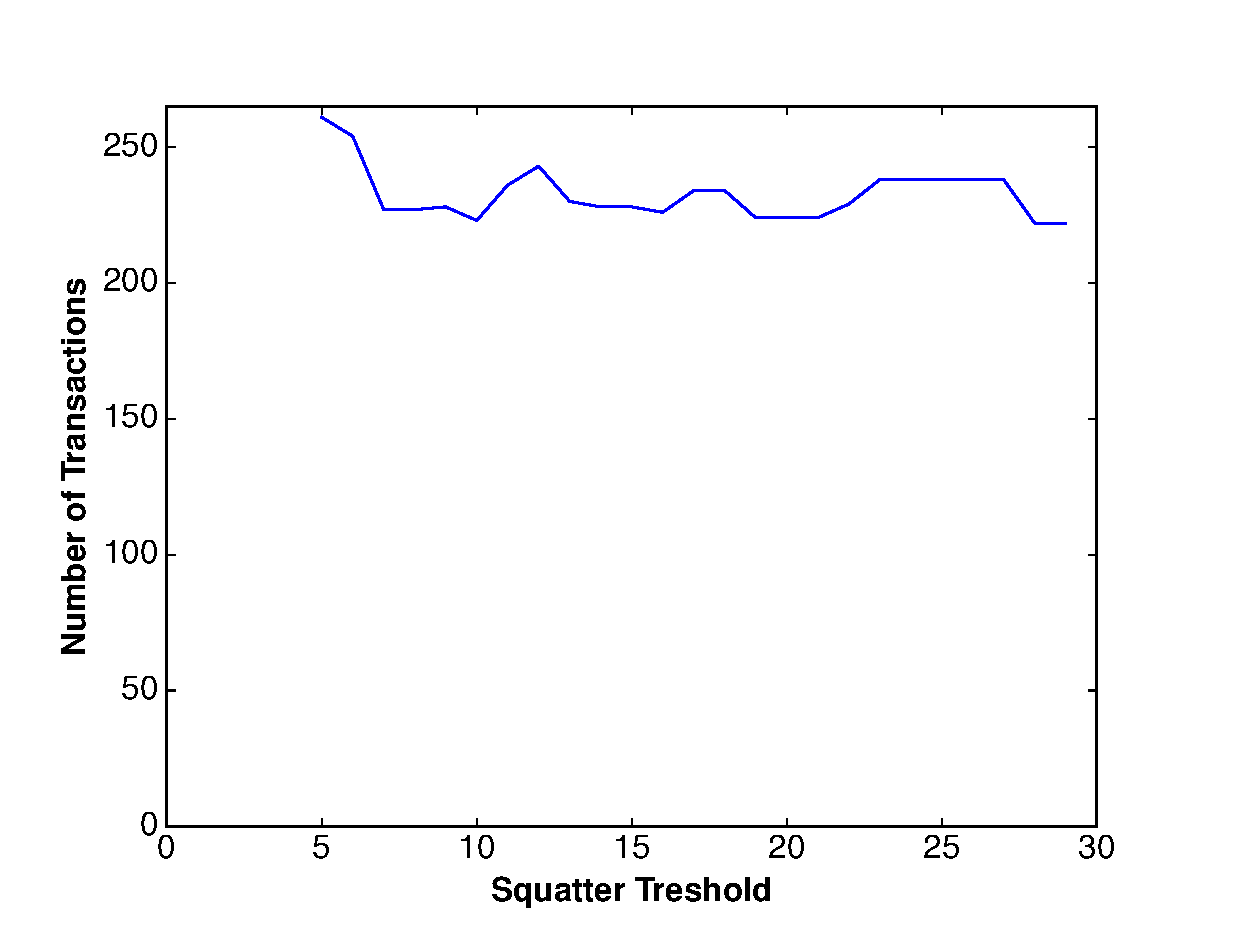
\includegraphics[width=0.9\columnwidth]{figures/transfers}
  \caption{Number of transfers detected based on squatting threshold. For each $n$ on the x-axis ($5 \leq n \leq 25$), we plot the number of squatter $\rightarrow$ non-squatter transactions detected if we characterize names whose values occur $n$ or more times as squatted.}
  \label{fig:percentSquatter}
\end{figure}

Although there doesn't seem to be a way to detect non-atomic name transfers generally, there is an important subclass of these transactions which can still be detected --- transfers from squatters to regular users. In the previous section we discussed our detection of squatters in the block chain which produces a list of values which with a high probability belong to squatters. Detecting transfers from squatters by finding names that change from one of these values to a value outside this set gives us a strategy to detect transfers.

We employ an additional criterion to eliminate false positives to tighten our upper bound. 
%Sometimes squatters update the value of their names, and thus a change from a squatter value may not represent the transfer of a name. To avoid picking up these updates as name transfers we restrict ourselves to selecting transactions that update the value of a name from a squatter value to a non-squatter value. 
If a name's value includes an info or email field and that stays the same in the updated value we can assume this is simply an update by the squatter. 

%Although this criterion is certainly not perfect, we believe that it has a fairly high success rate in revealing overall trends in name transfers.

Applying this analysis at various squatter threshold values, we see that the total number of squatter $\rightarrow$ non-squatter transactions detected holds at approximately 250 transactions. We emphasize that this value is likely an upper-bound since our criteria for reducing the number of transactions were quite conservative. 

To summarize, we would expect that given the high percentage of squatted .bit names, if there is a flourishing secondary market it would be dominated by sales from squatters to regular users. Yet we are able to upper bound the number of such transfers to about 250, a tiny fraction of the number of squatted names. Further, even though Namecoin supports a secure way to transfer names, we find strong evidence based on known tools supporting this functionality that its usage is very low.

\section{Analysis of Proposed Squatter Solutions}
\label{sec:analysis}

    Name squatting in Namecoin has been previously discussed as an issue facing the cryptocurrency. There have been several solutions proposed to alleviate the squatting issue by implementing new protocols or by placing additional fees on certain actions to either deter the actions of squatters or make it possible for a legitimate user to acquisition a desired name from a squatter if it increases the economic use of said name. In this section, we analyze some of the more popular methods, and discuss the costs to various individuals for each. 
    As it exists now, the only cost for an individual to register a name is the 0.01 NMC used to make the token, and then 0.01 NMC to cover two transactions fees (0.005 NMC each), one for the NAME\_NEW and one for the NAME\_FIRSTUPDATE transaction. Holding onto a name bares almost no cost with the owner only needing to pay 0.005 NMC as a transaction fee every time they post a NAME\_UPDATE transaction (which they need to do about once every 250 days). Losing a name doesn't cost a user anything, and the user gets gets the 0.01 NMC token back as a normal coin. 

\subsection{Adding a Cost to Updating Names}
    One of the most commonly suggested, and simplest, solutions to squatting is to add an associated fee with updating a name. The idea is that such a fee will not hinder a legitimate user very much, but will cause a squatter holding onto many domains to have to pay enough for the squatting to become financially infeasible. The reason that such a feature hasn't been implemented is because the Namecoin developers fear that the increased fees will disincentivise Namecoin adoption. Additionally, of the current squatters, some are benevolent and will give away names to users who have legitimate uses for the domains. Adding the renewal fees would punish these users who do not stand to gain monetarily from their efforts. This approach is very strong when it comes to deterring squatters who register thousands of domains. It is less effective against the type of squatter who registers just a few names that they think will be particularly valuable (like google.bit or poker.bit), or the type of squatter who is trying to squat on a name without the intent to sell, but just to hurt who they think the name would be valuable to.
For our analysis, we look into an update fee of 0.1 NMC. In this scenario, every time a user creates a NAME\_UPDATE transaction, a domain owner must burn 0.1 NMC for the transaction to be valid. Adding this fee wouldn't change the initial cost of registration, it would still be 0.02 NMC (0.01 from creating the token, and 2 transaction fees). The update fee will, however, change a user's cost on an update from 0.005 NMC to 0.105 NMC. Once the name expires, the user will again recoup their 0.01 NMC token that they attached to the name. 

\subsection{Varying Registration Costs Based on Name Lengths}
    Another commonly suggested solution is to vary the registration cost based on the length of the name. Shorter names are easier to remember, so the idea is they are generally worth more in practice and should cost more when they are registered. There have been various schemes suggested for the specifics on how the price should scale with name length, most of which resulting in exponentially decreasing costs for longer names. One issue with this approach is that the implicit assumption of this model, that shorter names are more valuable, may or may not actually reflect reality. Our results show that in the d/ namespace, more shorter names are taken, but this doesn't necessarily mean that they are more valuable. We speculate that a name like amazon.bit is probably more valuable than xyz.bit, and this wouldn't be reflected with this kind of pricing scheme.  This method does provide a good deterrent against squatters who are trying to claim many short names, but is rather ineffective against a squatter who is either trying to claim specific, valuable domain names, or hoard large quantities of longer domain names. 
    There exist many pricing protocols, but we have chosen to analyze the strategy outlined on the Namecoin Pricing wiki in more depth. According to this system, the prices depended on multipliers of an arbitrary price for different name lengths. 

\begin{figure*}
  \centering
  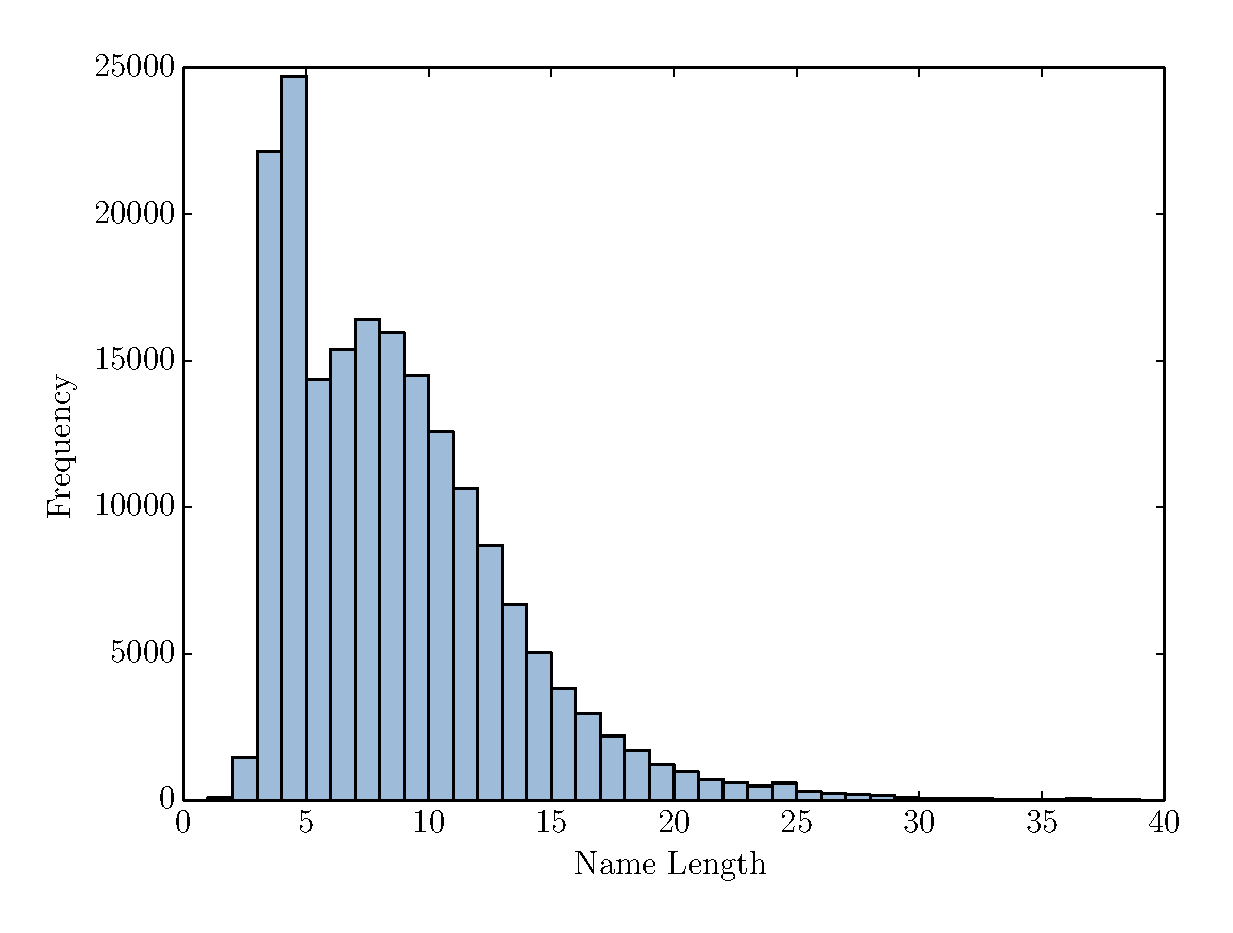
\includegraphics[width=0.95\textwidth]{figures/name_length_histogram}
  \caption{Length of Registered Names}
  \label{fig:nameLength}
\end{figure*}

\begin{table}[t]
  \centering
    \rowcolors{1}{}{lightgray}
  \begin{tabular}{| l | l |} \hline
    Length in Characters & Cost Multiplier \\
    1-3 & \( 5 x \) \\
    4-6 & \( 2 x \) \\
    7-14 & \( 1 x \) \\
    15-20 & \( \frac{1}{2} x \) \\
    21 + & minimum cost \\ \hline
  \end{tabular}
  \caption{Length based multipliers.}
\end{table}




    We use 0.5 NMC (could change) as the arbitrary price to be multiplied for our cost estimations. The update fees and the returned token are the same in this method as they are in the existing structure. The only change in cost is in the registration fee. In order to calculate what an average name would cost to register under this protocol, we have uniformly taken random names from the distribution of name length, and averaged the registration cost of these names. 



\subsection{Auctions}
    In this method for dealing with squatters, the Namecoin protocol could enforce that domain names are put up for auction on a periodic basis (perhaps every 52,000 blocks or about once/year). The protocol would allow for an auction after enough time has passed since the last auction, or since the NAME\_FIRSTUPDATE transaction for any given name. When an auction occurs, a name will become available and whomever is willing to pay the most for the domain name will get the name. In order to make it easier to retain a name, it has been suggested that the current owner should get some sort of advantage in the auction, so that the only need to bid some fraction of the highest bid in order to retain the name (let this be 1/100 for this discussion). If the current owner wins the auction, then they 'pay the network'. The cleanest way to do this is to burn the coins. Essentially, if the market cap of the currency doesn't change, then burning the coins from the auctions would uniformly increase the value of all the other remaining coins (burning too many coins can cause its own problems, too. Paying the network could also be done through other means, such as paying a random active address in the blockchain). The overall result should be that the fee paid for retaining a name should be spread out amongst other users of system. If, on the other hand, a new user wins the auction and bids more that 100 times the bid of the current owner of the name, the new user will gain the name, and the old owner will be the recipient of the auction coins. 
    An auction system like this has many disadvantages. The largest issue with this kind of squatting solution is that it erodes .bit's resistance to anti-censorship. One of the fundamental ideals of Namecoin and the .bit TLD is that it promotes freedom of speech, where a central authority is unable to censor content. Allowing a party to claim a domain as long as they are willing to pay enough undermines this concept. Periodic auctions would allow any large entity, such as an oppressive government, to easily seize names from any smaller entity that they want to silence. The counter argument here is that if a large entity seizes a smaller entities domain, the small entity would get paid a considerable sum-- in this case, 100 times what they were willing to bid to keep the domain. Whether or not the cash received by the censoring of the domain is worth more to the small entity than having the domain is a question that we do not explore.  An additional weakness of this system is that it can cause a legitimate user to have to pay lots of money in order to keep their domain every auction. Even with a large advantage, if owning a particular .bit domain is of great importance to an individual, then they can be forced to pay a large sum of money every auction. If "Business" is trying to hold onto business.bit, and business.bit is worth a considerable amount to them (say they get many online sales there), then a competitor to Business could bid some factor  less than what business.bit is worth to Business. Business isn't willing to part with business.bit for this amount of money, so they are forced to instead pay 1\% of what business.bit is worth every time there is an auction for their domain.
    Under this model, the initial cost a domain depends on how an individual acquires the domain. If they acquire the domain without an auction, then the cost is the same as it is in the existing protocol. Conversely, if an entity acquires a domain through the auction process, then the fee they will need to pay will depend on the value of the domain to whomever they are buying it from. If the seller is a squatter, the buyer will need to bid an amount equal to what the squatter thinks the domain is worth (the squatter will bid 1\% of what they think the domain is worth). Holding onto a domain in this model can be expensive; as discussed previously, every time there is an auction, the owner of a domain can be forced into paying 1\% of what the domain is worth to them, which could be a sizeable amount of money. Aside from the auction costs, there is still the small transaction fee that the owner will need to pay for every NAME\_UPDATE transaction. If a user lets their name expire, this situation is identical to the ones previously discussed, but if an individual loses control of a name because of an auction, they don't get their 0.01 NMC token back and they instead get the money from the auction. In this case, they receive an amount of money equal to the value of the domain to them. 

\subsection{Require an Escrow}
    Another proposed solution is to require a number of namecoins to be put into an escrow account when claiming a name. The money in escrow would be locked, so that the owner of the name is unable to spend that money, but once the owner loses or forfeits the name, the money in escrow is returned. The exact amount of money to be put into escrow is a debated topic. In one such model, the amount is decided by the owner of the name. In this situation, there would be an additional protocol designed to allow someone to take a name if they are willing to pay more money into an escrow account for said name than the current owner. If someone tries to place more money into escrow than the current owner (in an attempt to take the name), the current owner is notified and has a short grace period in which they can protect themselves by placing a larger amount of money in the escrow account. In order to prevent the the same problems and censorship erosion as seen in the case with auctions, there is a maximum allowed escrow and once a domain owner fills the escrow to this amount, the name becomes locked and it would be impossible for another user to seize for any amount of money (let this maximum value be 200 NMC). This provides reasonable financial protection against squatters who are trying to squat on thousands of domains, because a squatter such as this would need to fill the escrows for any of the domains that they are squatting that other people want. If a user out-escrows a squatter, this represents an ultimate failure in the eyes of the squatter because they lose the domain name and get paid nothing. The only way for a squatter to prevent this is to continue to fill their escrows for names that a user wants until the escrows are full. Once the squatter puts money into escrow, they can't remove it without losing the name, so eventually all of the escrows for all of the names users want would need to be full. This penalizes certain squatters more than others, in the sense that the squatter will always eventually get their coins back. A squatter that doesn't need access to their coins has no issue with locking up some huge fraction of them in escrow, because they will eventually get the coins back. A poorer squatter, on the other hand, who doesn't have enough coins to have some of them locked up for every domain they try to squat, will be forced to stop. 
    The cost of registering a name is now variable because a user can decide how much or little money they want to put into escrow. This has the advantage of being acceptable to many different types of users. A serious user who is only interested in having a few valued domains and doesn't want to risk losing their domains can easily pay to fill an escrow account for their domains. At the same time, a more casual user, who just wants some domain (but not a valuable domain) can still attain this domain while only owning a small number of coins. The cost of holding onto a domain is the same as it is in the present situation. Once a domain name is lost, a user will gain access to all the money locked into escrow for that name.     

\subsection{Cost Analysis}
    In order to compare the overall costs of the various models, we consider applying the cost assumptions outlined above to different users trying to hold onto domains for a period of 3 years. One user is a squatter who is trying to hold on to 1000 domains of variable length and value. Another is a squatter who is only trying to squat 5 particularly valuable names. The final two a legitimate users, one of which is looking to use a very specific, valued domain name, and the other is a user that just wants a domain, but doesn't really care what the domain is.


\begin{table*}[t]
  \centering
  \rowcolors{3}{}{lightgray}
  \begin{tabularx}{\linewidth}{| X | X | X | X | X |} \hline
    &  Squatter with 1000 domains & Squatter with a few valuable domains & User who wants any domain & User who wants a specific, valuable domain\\
\hline
    \multicolumn{5}{|c|}{\textbf{Registration Cost}} \\ \hline
Current System &  20 NMC & 0.1 NMC & 0.02 NMC & 0.02 NMC, or best offer from squatter \\
Increasing Update fee & 20 NMC & 0.1 NMC & 0.1 NMC & 0.02 NMC \\
Length based fees & 737.77 & 3.68 & 0.74 & 0.74 \\ 
Auctions & 20 NMC & 0.1 NMC & 0.1 NMC & Fee paid in Auction \\
Escrow & 200,000 NMC & 1,000 NMC & 0.02 NMC & 200 NMC \\ \hline

\multicolumn{5}{|c|}{\textbf{Longer term cost (3 years of Updates)}} \\ \hline
Current & 25 NMC & 0.125 NMC & 0.025 NMC & 0.025 NMC \\ 
Increasing Update fee & 500 NMC & 2.5 NMC & 0.5 NMC & 0.5 NMC \\ 
Length based fees & 25 NMC & 0.125 NMC & 0.025 NMC & 0.025 NMC \\ 
Auctions & & & 1 \% of what domain is worth to user & 1 \% of what domain is worth to user \\ 
Escrow & 25 NMC & 0.125 NMC & 0.025 NMC & 0.025 NMC \\ \hline

\multicolumn{5}{|c|}{\textbf{Refund Upon Losing Name}} \\ \hline
Current & 10 NMC & 0.05 NMC & 0.01 NMC & 0.01 NMC \\
Increasing Update fee & 10 NMC & n0.05 NMC & 0.01 NMC & 0.01 NMC \\
Length based fees & 10 NMC & 0.05 NMC & 0.01 NMC & 0.01 NMC \\
Auctions & & & What the domain is worth to user & What the domain is worth to user \\ \hline
  \end{tabularx}
  \caption{Cost comparison of the various anti-squatter mechanisms.}
\end{table*}



\section{Related Work}
\label{sec:related}

Here we discuss attempts besides Namecoin at decentralized cryptocurrency-based namespaces or domain-name systems and more broadly in technologies that utilize the block chain.

Bitshares is another altcoin that includes proposals for a namespace as one of its goals \cite{bitsharesdns}. Emercoin recently emerged as a Namecoin competitor \cite{emercoin}. 

More broadly, the ability to publish messages to the block chain immediately allows a variety of applications. Physical property, shares of stocks, bonds, or any other real asset can be digitally represented on the block chain. Overlay protocols such as Mastercoin and Colored Coins specify a syntax and semantics for such digital representations \cite{mastercoinspec, rosenfeld2012overview}. CommitCoin allows for putting hash commitments on the Bitcoin block chain in order to timestamp data in a trustless manner \cite{clark2012commitcoin}.

There are a number of more complex applications that require additional primitives. Financial derivatives are contracts whose value depends, in some mutually agreed-upon way, on the price (or movements in price) of an underlying asset. Implementing derivatives of digital assets, then, requires user-defined logic (or scripts) for transaction validation. This can be accomplished via an altcoin with a flexible scripting language such as Ethereum \cite{ethereumwhitepaper}. Furthermore, since derivatives depend on prices, scripts that implement them require access to price feeds as input. Otherwise, it requires a trusted third party (known by a Bitcoin address) to regularly publish suitably encoded, signed price statements reflecting external reality. These can be published directly to the block chain or distributed off-chain and only added to the block chain when needed to redeem an asset. More generally, such entities could publish any data feed representing news or other events.

Bitcoin can act as a platform for fair secure multiparty computation \cite{andrychowicz2014secure, bentov2014use, kumaresan2014use}. These are SMC protocols augmented with Bitcoin operations, e.g., a payment from one participant to another, or a deposit.

Finally, a set of related ideas known as decentralized autonomous organizations (among several other names) has stirred considerable excitement in the community recently. These combine several primitives discussed above --- digital assets, long-lived scripts implementing arbitrary logic governing those assets, data feeds, and out-of-band communication. Some proposals for DAOs incorporate human input in various forms: one is a decentralized agent farming out computationally intractable tasks to humans \cite{buterindao}. Another is voting by shareholders of decentralized agents to enable modifications to the logic (i.e., script). 

% As with any input external to the block chain, these must be implemented using data feeds.

% The block chain has been proposed as a stratum for building technologies and mechanisims beyond storing financial transactions. Hash commitments appear in the Namecoin protocol for registering new names. In  \cite{bonneau2014decentralizing} the authors describe how to use the block chain to create prediction markets and order books.

\section{Conclusion}
\label{sec:conclusion}


%% Bibliography
%\vspace{-1ex}
%\linespread{1.0}
%\setlength{\bibsep}{1pt}
%\footnotesize
\small
\bibliographystyle{unsrtnat}
% \bibliographystyle{abbrvnat}
\bibliography{local}

\clearpage
\appendix
\section{List of .bit domains with content and without ICANN hostname}
\begin{itemize}
\item alt-freedom.bit
\item bangkokgroup.bit
\item bitcoinpl.bit
\item bitcoinquotes.bit
\item carnicominstitutemirror.bit
\item changepurse.bit
\item columbo.bit
\item darkfur93.bit
\item dcinvestments.bit
\item dealing.bit
\item deathrowdemocracy.bit
\item dot-bit.bit
\item dotbitkittypix.bit
\item feens.bit
\item hewgill.bit
\item hosting.bit
\item kk-cabrio.bit
\item lapan.bit
\item medicinalgenomics.bit
\item megabrutal.bit
\item michail.bit
\item mikeward.bit
\item namecoin-test-suite-1.bit
\item onemillionpixels.bit
\item peterboswell.bit
\item rmgx.bit
\item tuler.bit
\item wikimouto.bit
\end{itemize}




\end{document}

